\section{Introduction}
\label{sec:icra21_intro}

Mobile manipulation is the field of robotics in which a mobile robot's locomotion ability is combined with the manipulation ability of a robotic arm. However, conventional trajectory optimization methods dealing with such systems often dramatically reduce flexibility by decoupling planning for the base and the arm. Motion for both parts then need to be synchronized or are executed sequentially. Both synchronization and sequencing limit the ability of the robot to perform complex tasks, and it was shown that decoupled and sequenced approaches show significantly higher operational times \cite{Thakar2018,Thakar2019}. 
% Limitations with coupling
Yet, solving the whole-body trajectory optimization problem is challenging due to a large number of degrees of freedom (e.g., 10 for the robot used in our experiments and shown in Fig. \ref{fig:real_robot}). Moreover, dynamic and unstructured environments have not been addressed in a coupled approach yet.
% MPC and limitations
Such environments have been extensively investigated for autonomous vehicles (e.g., mobile robots navigating through human crowds \cite{Trautman2010, Chen2019a}, drones in cluttered environments \cite{Liu2017, Tordesillas2019}). In the context of autonomous vehicles, model predictive control (MPC) can effectively incorporate future evolutions of the environment \cite{Brito2019}.
% MPC FOR MM
A coupled MPC scheme for mobile manipulators was introduced in \cite{Avanzini2015}, where locomotion and manipulation were softly decoupled through dynamic weight-setting. Dynamic obstacles were not considered, and the method suffered from increasing computational costs as the environment becomes more densely populated \cite{Avanzini2018}.
More specifically, collision avoidance in an unstructured environment typically results in many inequality constraints that scale with the number of obstacles.
%
%
\begin{figure}[ht]
  \centering
  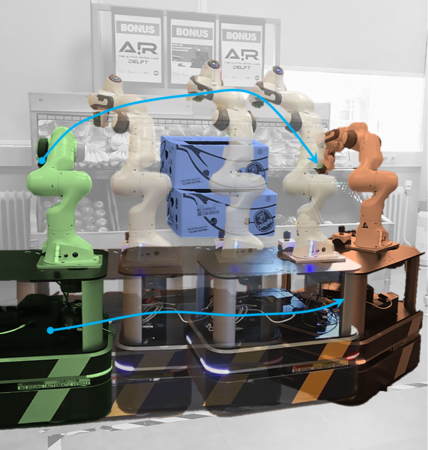
\includegraphics[width=0.3\linewidth]{real/real_traj_small.png}
  \caption{Mobile manipulator performing a pick \& place task using whole-body trajectory optimization with our coupled MPC formulation.}%
  \label{fig:real_robot}
\end{figure}
%

In this work, we propose a whole-body trajectory optimization, sometimes referred to as MPC, using convex region decomposition of the free space on multiple kinematic chain links for collision avoidance with static obstacles.  As a result, the number of inequality constraints remains constant regardless of the number of obstacles, allowing continuous control of the arm and the base to navigate through unstructured environments. Dynamic sphere-shaped obstacle avoidance is included using stage-dependent sphere-to-sphere inequality constraints.

Experimental results demonstrated that operational time is reduced considerably when using whole-body trajectory optimization. Computational costs for the optimization solver were independent of the number of obstacles present in the environment. Single dynamic obstacles moving at a constant velocity could be avoided successfully.

